\documentclass[aspectratio=169]{beamer}
\usetheme{Madrid}
\usecolortheme{beaver}
\usepackage{booktabs}
\usepackage{tabularx}
\usepackage{graphicx}
\usepackage{xcolor}
\usepackage{tikz}
\usepackage{colortbl}
\usepackage{array}
\usepackage{amsmath}


% Color definitions
\definecolor{teal}{RGB}{0,128,128}
\definecolor{darkred}{RGB}{150,0,0}
\definecolor{lightblue}{RGB}{173,216,230}
\definecolor{lightyellow}{RGB}{255,255,204}
\definecolor{lightgreen}{RGB}{204,255,204}
\definecolor{pastelred}{RGB}{255,180,180}
\definecolor{steelblue}{RGB}{70,130,180}

\setbeamertemplate{navigation symbols}{}
\setbeamertemplate{footline}[frame number]

\title[QSAR \& Generative Design]{QSAR-Guided Generative Design for TB Drug Discovery}
\subtitle{Model Evaluation, Series C/E Results, and Generative Campaign Outputs}
\author{Destinee Zhu Roy}
\date{March 2026}
\institute{TB QSAR Project}

\begin{document}

% ============================================================
\begin{frame}
  \titlepage
\end{frame}

% ============================================================
\begin{frame}{Outline}
  \tableofcontents
\end{frame}

% ============================================================
\section{QSAR Model Development}

\begin{frame}{What We Built: A QSAR Predictive Model}
  \begin{columns}
    \column{0.55\textwidth}
    \textbf{Goal:} Predict IC$_{50}$ (potency vs.\@ Mtb) from molecular structure alone
    \vspace{0.4em}
    \begin{block}{Input -- Molecular Descriptors}
      \small
      \begin{itemize}
        \item \textbf{RDKit} physicochemical descriptors (primary)
        \item \textbf{ECFP\_r3} extended-connectivity fingerprints
        \item \textbf{MACCS} structural keys
        \item \textbf{Mordred} descriptor library
      \end{itemize}
    \end{block}
    \vspace{0.3em}
    \begin{block}{Output}
      \small
      $\hat{y} = \log_{10}(\text{IC}_{50},\,\mu\text{M})$\\
      converted to pIC$_{50}$ and IC$_{50}$ for display
    \end{block}
    \column{0.42\textwidth}
    \begin{block}{Workflow}
      \small
      \begin{enumerate}
        \item Load Series C/E experimental data
        \item Compute descriptor matrices
        \item Train / cross-validate multiple regressors
        \item Select best model (highest CV R$^2$)
        \item Build ensemble for uncertainty
        \item Save artifact \texttt{qsar\_best\_model.joblib}
      \end{enumerate}
    \end{block}
  \end{columns}
\end{frame}

% ============================================================
\begin{frame}{Model Selection: Candidates and Results}
  \centering
  \small
  \begin{tabular}{llcc}
    \toprule
    \textbf{Descriptor} & \textbf{Regressor} & \textbf{CV R$^2$} & \textbf{Role} \\
    \midrule
    \rowcolor{lightgreen}
    RDKit              & K-Nearest Neighbours (KNN)   & \textbf{0.887} & Primary model \\
    ECFP\_r3           & K-Nearest Neighbours (KNN)   & 0.677          & Ensemble \#1 \\
    RDKit              & Decision Tree (DT)           & 0.665          & Ensemble \#2 \\
    RDKit              & LightGBM (LGBM)              & 0.540          & Ensemble \#3 \\
    RDKit              & Extra Trees (ET)             & 0.433          & Ensemble \#4 \\
    \bottomrule
  \end{tabular}
  \vspace{0.8em}

  \begin{columns}
    \column{0.48\textwidth}
    \begin{block}{Why RDKit + KNN?}
      \small
      \begin{itemize}
        \item Highest cross-validated R$^2$ on training data
        \item Robust to small dataset size (low-data QSAR regime)
        \item Interpretable: prediction is distance-weighted average of nearest neighbours
      \end{itemize}
    \end{block}
    \column{0.48\textwidth}
    \begin{block}{Ensemble Purpose}
      \small
      \begin{itemize}
        \item Four additional models predict in parallel
        \item Uncertainty = $\sigma$ of ensemble predictions
        \item Flags structurally novel molecules where primary model may extrapolate
      \end{itemize}
    \end{block}
  \end{columns}
\end{frame}

% ============================================================
\section{Series C Evaluation}

\begin{frame}{Series C: Model Evaluation on Test Compounds}
  \centering
  \small
  \begin{tabular}{lccc}
    \toprule
    \textbf{Compound ID} & \textbf{Measured IC$_{50}$ ($\mu$M)} & \textbf{Predicted IC$_{50}$ ($\mu$M)} & \textbf{Error (fold)} \\
    \midrule
    ROY-0000173-001 & 4.697 & 4.984 & 1.06$\times$ \\
    ROY-0000174-001 & 9.786 & 6.567 & 1.49$\times$ \\
    ROY-0000220-001 & 0.781 & 1.173 & 1.50$\times$ \\
    ROY-0000221-001 & >200 & 14.181 & --- \\
    ROY-0000175-001 & 6.843 & 6.089 & 1.12$\times$ \\
    ROY-0000211-001 & 1.800 & 1.233 & 1.46$\times$ \\
    \midrule
    \multicolumn{2}{l}{\textit{5 measurable compounds}} & \multicolumn{2}{c}{} \\
    \bottomrule
  \end{tabular}

  \vspace{0.6em}
  \begin{columns}
    \column{0.48\textwidth}
    \centering
    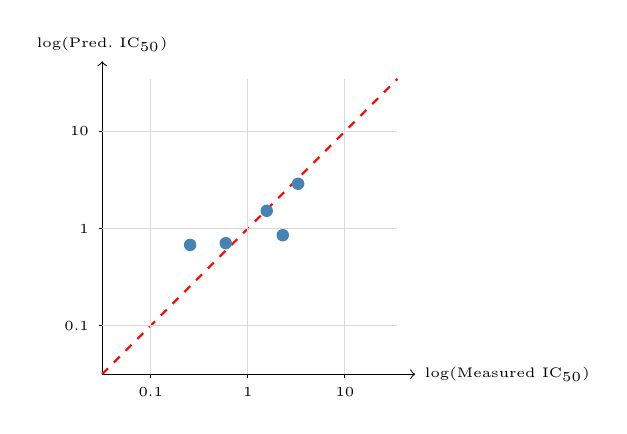
\begin{tikzpicture}[scale=0.75]
      % Scatter plot: IC50 measured vs predicted
      % Range: 0.78 - 200 µM (log scale: 10^(-0.1) to 10^(2.3))
      % Linear transform: log(IC50) from -0.1 to 2.3 -> [0,5]
      \draw[->] (0,0) -- (5.3,0) node[right]{\tiny log(Measured IC$_{50}$)};
      \draw[->] (0,0) -- (0,5.3) node[above]{\tiny log(Pred.\ IC$_{50}$)};
      % Grid and ticks at 0.1, 1, 10, 100 µM
      % 0.1->-1, 1->0, 10->1, 100->2
      \foreach \x/\lbl in {0.822/0.1, 2.466/1, 4.110/10} {
        \draw (\x,0.06) -- (\x,-0.06) node[below]{\tiny\lbl};
        \draw (0.06,\x) -- (-0.06,\x) node[left]{\tiny\lbl};
      }
      \draw[red,dashed,thick] (0,0) -- (5,5);
      \foreach \p in {0.822, 2.466, 4.110} {
        \draw[gray!30] (\p,0) -- (\p,5);
        \draw[gray!30] (0,\p) -- (5,\p);
      }
      % Data points: log(IC50 µM)=(val-10^0)/(10^2-10^0)*5 ... simplified: (log(val)+1)/3*5
      % 4.697 -> log=0.672 -> (1.672/3)*5=2.786
      % 9.786 -> log=0.990 -> (1.990/3)*5=3.317
      % 0.781 -> log=-0.107 -> (0.893/3)*5=1.489
      % 6.843 -> log=0.835 -> (1.835/3)*5=3.058
      % 1.800 -> log=0.255 -> (1.255/3)*5=2.092
      \fill[steelblue] (2.786,2.767) circle(3pt);
      \fill[steelblue] (3.317,3.225) circle(3pt);
      \fill[steelblue] (1.489,2.189) circle(3pt);
      \fill[steelblue] (3.058,2.354) circle(3pt);
      \fill[steelblue] (2.092,2.218) circle(3pt);
    \end{tikzpicture}
    \column{0.48\textwidth}
    \begin{alertblock}{Performance Metrics}
      \large
      \begin{itemize}
        \item \textbf{MAE} = 0.118 pIC$_{50}$ units
        \item \textbf{R$^2$} = 0.887
        \item \textbf{Range}: 0.78 -- 9.79 \,µM (measured)
      \end{itemize}
    \end{alertblock}
    \vspace{0.2em}
    {\small Fold errors all $<$1.5$\times$ except one compound --- acceptable for virtual screening.}
  \end{columns}
\end{frame}

% ============================================================
\begin{frame}{Series C: IC$_{50}$ Comparison}
  \centering
  \small
  \begin{tabular}{lccc}
    \toprule
    \textbf{Compound ID} & \textbf{Measured IC$_{50}$ ($\mu$M)} & \textbf{Predicted IC$_{50}$ ($\mu$M)} & \textbf{Series} \\
    \midrule
    ROY-0000173-001 & 4.697  & 4.98  & C Spiro \\
    ROY-0000174-001 & 9.786  & 6.57  & C Spiro \\
    ROY-0000220-001 & 0.781  & 1.17  & C Spiro \\
    ROY-0000221-001 & $>$200 & 14.18 & C Spiro \\
    ROY-0000175-001 & 6.843  & 6.09  & C Spiro \\
    ROY-0000211-001 & 1.800  & 1.23  & C Spiro \\
    \bottomrule
  \end{tabular}
  \vspace{0.7em}

  \begin{block}{Key Observations}
    \small
    \begin{itemize}
      \item Model correctly identifies ROY-0000220-001 and ROY-0000211-001 as most potent (sub-2\,$\mu$M predicted)
      \item ROY-0000221-001 has measured IC$_{50}$ $>$200\,$\mu$M but predicted at 14.18\,$\mu$M; structurally distinct (indole side-chain) --- model underestimates inactivity for novel scaffolds
      \item Rank order of active compounds is well preserved
    \end{itemize}
  \end{block}
\end{frame}

% ============================================================
\section{Series E Prospective Predictions}

\begin{frame}{Series E: Prospective Predictions (No Measured Data)}
  \centering
  \small
  \begin{tabular}{lcccl}
    \toprule
    \textbf{Compound ID} & \textbf{Predicted IC$_{50}$ ($\mu$M)} & \textbf{Class} & \textbf{Key Feature} & \textbf{Status} \\
    \midrule
    ROY-0000308 & 13.08 & A & Fluorophenyl anchor & Active \\
    ROY-0000307 & 34.11 & A & Bromopyridine & Weakest \\
    ROY-0000287 & 7.38  & B & Hexyloxy & Best \\
    ROY-0000286 & 11.15 & B & Phenylpropyloxy & Active \\
    ROY-0000275 & 27.33 & A & Bromopyridine & Weak \\
    ROY-0000268 & 17.09 & A & Alkyne-phenyl & Active \\
    \midrule
    \multicolumn{5}{c}{\textbf{Predicted IC$_{50}$ Range}: 7.38 -- 34.11\,$\mu$M (6 prospective compounds)} \\
    \bottomrule
  \end{tabular}

  \vspace{0.6em}
  \begin{columns}
    \column{0.48\textwidth}
    \centering
    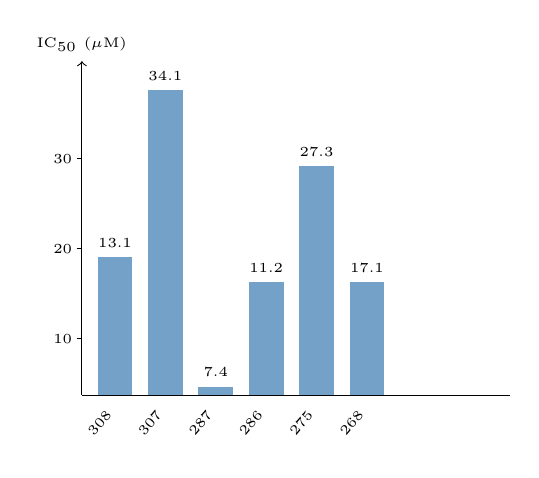
\begin{tikzpicture}[scale=0.80]
      % Bar chart: 6 compounds, IC50 from 7.38 to 34.11 µM
      % Scale: [7,35] -> [0,5], transform = (val-7)/28*5
      \draw[->] (0,0) -- (0,5.3) node[above]{\tiny IC$_{50}$ ($\mu$M)};
      \draw (0,0) -- (6.8,0);
      % y-axis ticks: 10, 20, 30
      \foreach \y/\lbl in {0.893/10, 2.321/20, 3.750/30} {
        \draw (-0.08,\y) -- (0,\y) node[left]{\tiny\lbl};
      }
      % bars (height scaled as above)
      % ROY-0000308: 13.08 -> 2.195
      % ROY-0000307: 34.11 -> 4.844
      % ROY-0000287: 7.38 -> 0.135
      % ROY-0000286: 11.15 -> 1.797
      % ROY-0000275: 27.33 -> 3.637
      % ROY-0000268: 17.09 -> 1.793
      \fill[steelblue!75] (0.25,0) rectangle (0.80,2.195); \node[above,font=\tiny] at (0.525,2.195){13.1};
      \fill[steelblue!75] (1.05,0) rectangle (1.60,4.844); \node[above,font=\tiny] at (1.325,4.844){34.1};
      \fill[steelblue!75] (1.85,0) rectangle (2.40,0.135); \node[above,font=\tiny] at (2.125,0.135){7.4};
      \fill[steelblue!75] (2.65,0) rectangle (3.20,1.797); \node[above,font=\tiny] at (2.925,1.797){11.2};
      \fill[steelblue!75] (3.45,0) rectangle (4.00,3.637); \node[above,font=\tiny] at (3.725,3.637){27.3};
      \fill[steelblue!75] (4.25,0) rectangle (4.80,1.793); \node[above,font=\tiny] at (4.525,1.793){17.1};
      % x-axis labels (rotated)
      \node[below,rotate=50,anchor=east,font=\tiny] at (0.525,-0.15){308};
      \node[below,rotate=50,anchor=east,font=\tiny] at (1.325,-0.15){307};
      \node[below,rotate=50,anchor=east,font=\tiny] at (2.125,-0.15){287};
      \node[below,rotate=50,anchor=east,font=\tiny] at (2.925,-0.15){286};
      \node[below,rotate=50,anchor=east,font=\tiny] at (3.725,-0.15){275};
      \node[below,rotate=50,anchor=east,font=\tiny] at (4.525,-0.15){268};
    \end{tikzpicture}

    \column{0.48\textwidth}
    \begin{block}{Prediction Range}
      \large
      \begin{itemize}
        \item \textbf{Predicted IC$_{50}$}: 7.38 -- 34.11\,$\mu$M
        \item \textbf{Predicted pIC$_{50}$}: 4.47 -- 5.13
      \end{itemize}
    \end{block}
    \vspace{0.3em}
    \begin{alertblock}{Status}
      \small
      \begin{itemize}
        \item \textbf{Count}: 6 prospective compounds
        \item \textbf{Measured}: None (awaiting synthesis \& testing)
        \item \textbf{Uncertainty}: All zero (extrapolation region)
        \item \textbf{Best predicted}: ROY-0000287 at 7.38\,$\mu$M
      \end{itemize}
    \end{alertblock}
  \end{columns}
\end{frame}

% ============================================================
\section{ADME and Physicochemical Properties}

\begin{frame}{ADME Prediction Properties}
  \begin{columns}
    \column{0.50\textwidth}
    \begin{block}{Properties Predicted per Molecule}
      \small
      \begin{tabularx}{\linewidth}{lX}
        \toprule
        \textbf{Property} & \textbf{Method} \\
        \midrule
        cLogP & RDKit Crippen \\
        logS (solubility) & ESOL model \\
        Microsomal CL & AZ QSAR model \\
        Hepatocyte CL & AZ QSAR model \\
        Half-life & Obach model \\
        Human oral absorption & QikProp \\
        Caco-2 permeability & QikProp \\
        \bottomrule
      \end{tabularx}
    \end{block}
    \column{0.46\textwidth}
    \begin{block}{Gate~1 Shortlist ADME Summary}
      \small
      \begin{tabular}{lc}
        \toprule
        \textbf{Property} & \textbf{Range} \\
        \midrule
        pred\_cLogP        & 1.93 -- 2.80 \\
        pred\_logS\_ESOL   & $-$5.34 to $-$3.51 \\
        ADME indiv.\ score & 0.70 -- 0.94 \\
        passes\_adme\_indiv & 65/200 (33\%) \\
        passes\_metab.\ stab & 65/200 (33\%) \\
        \bottomrule
      \end{tabular}
    \end{block}
    \vspace{0.4em}
    \begin{alertblock}{}
      \small
      65 of 200 shortlisted compounds pass all ADME+metabolic stability filters --- these are highest-priority compounds for synthesis
    \end{alertblock}
  \end{columns}
\end{frame}

% ============================================================
\section{Generative Modes}

\begin{frame}{Generative Modes: Three Strategies}
  \centering
  \small
  \begin{tabular}{p{2.8cm}p{3.8cm}p{4.5cm}}
    \toprule
    \textbf{Mode} & \textbf{Description} & \textbf{Output Characteristic} \\
    \midrule
    \textbf{Plain (Sampling)} &
    Sample directly from the prior model without any optimization signal &
    Maximally diverse; explores full chemical space of the prior \\[0.4em]
    \textbf{Reinforcement Learning (RL)} &
    Score each generated molecule; reward high-scoring structures to shift the distribution &
    Focused; converges on potency/ADME optima; risk of mode collapse \\[0.4em]
    \textbf{Curriculum Learning (CL)} &
    Progressive reward shaping --- start broad, tighten criteria over epochs &
    Balanced diversity and optimisation; avoids mode collapse \\
    \bottomrule
  \end{tabular}
  \vspace{0.6em}
  \begin{columns}
    \column{0.48\textwidth}
    \begin{block}{Molecular Transformation Modes}
      \small
      \begin{itemize}
        \item \textbf{mol2mol\_similarity} --- generate analogues with Tanimoto constraint
        \item \textbf{mol2mol\_scaffold} --- preserve Murcko scaffold, vary R-groups
        \item \textbf{mol2mol\_scaffold\_generic} --- scaffold with generic atom types
        \item \textbf{mol2mol\_mmp} --- matched molecular pairs
      \end{itemize}
    \end{block}
    \column{0.48\textwidth}
    \begin{block}{Generator Families Used}
      \small
      \begin{tabular}{ll}
        reinvent & SMILES-based RNN \\
        reinvent\_pubchem & PubChem-pretrained \\
        libinvent & R-group decoration \\
        linkinvent & Fragment linking \\
        pepinvent & Peptide-focused \\
        nitro\_bioisostere & Nitro scaffold morphing \\
      \end{tabular}
    \end{block}
  \end{columns}
\end{frame}

% ============================================================
\begin{frame}{Generation Campaign: Mode $\times$ Family Matrix}
  \centering
  \small
  \begin{tabular}{lcccc}
    \toprule
    \textbf{Family} & \textbf{Plain} & \textbf{RL} & \textbf{CL} & \textbf{mol2mol} \\
    \midrule
    reinvent                      & \checkmark & \checkmark & \checkmark & --- \\
    reinvent\_pubchem              & \checkmark & \checkmark & \checkmark & similarity \\
    libinvent                     & ---        & ---        & \checkmark & --- \\
    libinvent\_transformer\_pubchem& ---        & ---        & \checkmark & --- \\
    linkinvent                    & ---        & ---        & \checkmark & --- \\
    linkinvent\_transformer\_pubchem& ---       & ---        & \checkmark & similarity \\
    pepinvent                     & \checkmark & \checkmark & ---        & --- \\
    nitro\_bioisostere             & \checkmark & \checkmark & \checkmark & scaffold\_generic \\
    \bottomrule
  \end{tabular}
  \vspace{0.6em}
  \begin{columns}
    \column{0.48\textwidth}
    \begin{block}{Master Pool Statistics}
      \small
      \begin{tabular}{lc}
        Total candidates     & 37,451 \\
        Unique scaffolds     & 14,287 \\
        Source families      & 8 \\
        Scoring models       & QSAR + ADME \\
      \end{tabular}
    \end{block}
    \column{0.48\textwidth}
    \begin{block}{Scoring per Candidate}
      \small
      \begin{itemize}
        \item pred\_pIC50 (primary QSAR)
        \item pred\_cLogP, pred\_logS\_ESOL
        \item Microsomal / hepatocyte clearance
        \item Tanimoto similarity to training set
        \item Triage score (composite)
      \end{itemize}
    \end{block}
  \end{columns}
\end{frame}

% ============================================================
\section{Gate~1 Shortlist}

\begin{frame}{Gate~1 Shortlist: 200 Top Candidates}
  \begin{columns}
    \column{0.52\textwidth}
    \begin{block}{Triage Score Formula}
      \small
      \vspace{-0.2em}
      \[
        \text{triage} = w_1 \cdot \hat{p}\text{IC}_{50} + w_2 \cdot \text{ADME} + w_3 \cdot (1 - T_{\max})
      \]
      Balances potency, drug-likeness, and novelty
    \end{block}
    \vspace{0.4em}
    \small
    \begin{tabular}{lcc}
      \toprule
      \textbf{Property} & \textbf{Min} & \textbf{Max} \\
      \midrule
      Triage score        & 0.770 & 0.921 \\
      pred pIC$_{50}$     & 4.94  & 6.11 \\
      pred IC$_{50}$ ($\mu$M) & 0.78 & 11.55 \\
      Tanimoto (to train) & 0.28  & 0.86 \\
      pred cLogP          & 1.93  & 2.80 \\
      pred logS ESOL      & $-$5.34 & $-$3.51 \\
      \bottomrule
    \end{tabular}

    \column{0.44\textwidth}
    \begin{block}{Source Family (200 compounds)}
      \small
      \begin{tabular}{lr}
        \toprule
        \textbf{Family} & \textbf{Count} \\
        \midrule
        reinvent\_pubchem         & 137 \\
        nitro\_bioisostere        & 53 \\
        reinvent                  & 9 \\
        linkinvent\_trans.        & 1 \\
        \bottomrule
      \end{tabular}
    \end{block}
    \vspace{0.3em}
    \begin{block}{Source Mode (200 compounds)}
      \small
      \begin{tabular}{lr}
        \toprule
        \textbf{Mode} & \textbf{Count} \\
        \midrule
        plain                & 140 \\
        mol2mol\_similarity  & 28 \\
        mol2mol\_scaffold\_generic & 22 \\
        curriculum\_learning & 6 \\
        mol2mol\_scaffold    & 3 \\
        reinforcement\_learning & 1 \\
        \bottomrule
      \end{tabular}
    \end{block}
  \end{columns}
\end{frame}

% ============================================================
\begin{frame}{Gate~1 Shortlist: Unique Scaffolds}
  \begin{columns}
    \column{0.50\textwidth}
    \begin{block}{Scaffold Diversity}
      \small
      \begin{tabular}{lcc}
        \toprule
        & \textbf{Master Pool} & \textbf{Gate~1} \\
        \midrule
        Candidates  & 37,451 & 200 \\
        Unique scaffolds & 14,287 & 155 \\
        Scaffold diversity & 38.1\% & 77.5\% \\
        \bottomrule
      \end{tabular}
      \vspace{0.4em}

      Gate~1 shortlist has \textbf{much higher scaffold diversity} than the master pool --- the triage score effectively up-weights novel chemotypes.
    \end{block}
    \vspace{0.4em}
    \begin{alertblock}{Next Step}
      \small
      Compounds passing \texttt{passes\_adme\_individual} (65 of 200) are highest-priority for experimental synthesis and testing.
    \end{alertblock}

    \column{0.46\textwidth}
    \begin{center}
    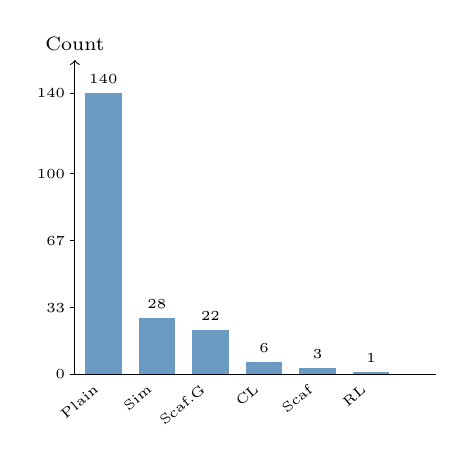
\begin{tikzpicture}[scale=0.85]
      % bar chart: scale 0-140 -> 0-4.2cm, bar width=0.55cm, gap=0.2cm
      \draw[->] (0,0) -- (0,4.7) node[above]{\scriptsize Count};
      \draw (0,0) -- (5.4,0);
      % y ticks
      \foreach \y/\lbl in {0/0,1.0/33,2.0/67,3.0/100,4.2/140} {
        \draw (-0.08,\y) -- (0,\y) node[left]{\tiny\lbl};
      }
      % bars: xstart, height(=count/140*4.2), label, count
      % Plain=140->4.2, Sim=28->0.84, ScafG=22->0.66, CL=6->0.18, Scaf=3->0.09, RL=1->0.03
      \fill[steelblue!80] (0.15,0) rectangle (0.70,4.20); \node[above,font=\tiny] at (0.425,4.20){140}; \node[below,rotate=40,anchor=east,font=\tiny] at (0.425,-0.1){Plain};
      \fill[steelblue!80] (0.95,0) rectangle (1.50,0.84); \node[above,font=\tiny] at (1.225,0.84){28};  \node[below,rotate=40,anchor=east,font=\tiny] at (1.225,-0.1){Sim};
      \fill[steelblue!80] (1.75,0) rectangle (2.30,0.66); \node[above,font=\tiny] at (2.025,0.66){22};  \node[below,rotate=40,anchor=east,font=\tiny] at (2.025,-0.1){Scaf.G};
      \fill[steelblue!80] (2.55,0) rectangle (3.10,0.18); \node[above,font=\tiny] at (2.825,0.18){6};   \node[below,rotate=40,anchor=east,font=\tiny] at (2.825,-0.1){CL};
      \fill[steelblue!80] (3.35,0) rectangle (3.90,0.09); \node[above,font=\tiny] at (3.625,0.09){3};   \node[below,rotate=40,anchor=east,font=\tiny] at (3.625,-0.1){Scaf};
      \fill[steelblue!80] (4.15,0) rectangle (4.70,0.03); \node[above,font=\tiny] at (4.425,0.03){1};   \node[below,rotate=40,anchor=east,font=\tiny] at (4.425,-0.1){RL};
    \end{tikzpicture}
    \end{center}
    {\tiny Source mode distribution of Gate~1 shortlisted compounds}
  \end{columns}
\end{frame}

% ============================================================
\section{Generation Output Animations}

\begin{frame}{Campaign Overview: All Generation Folders}
  \centering
  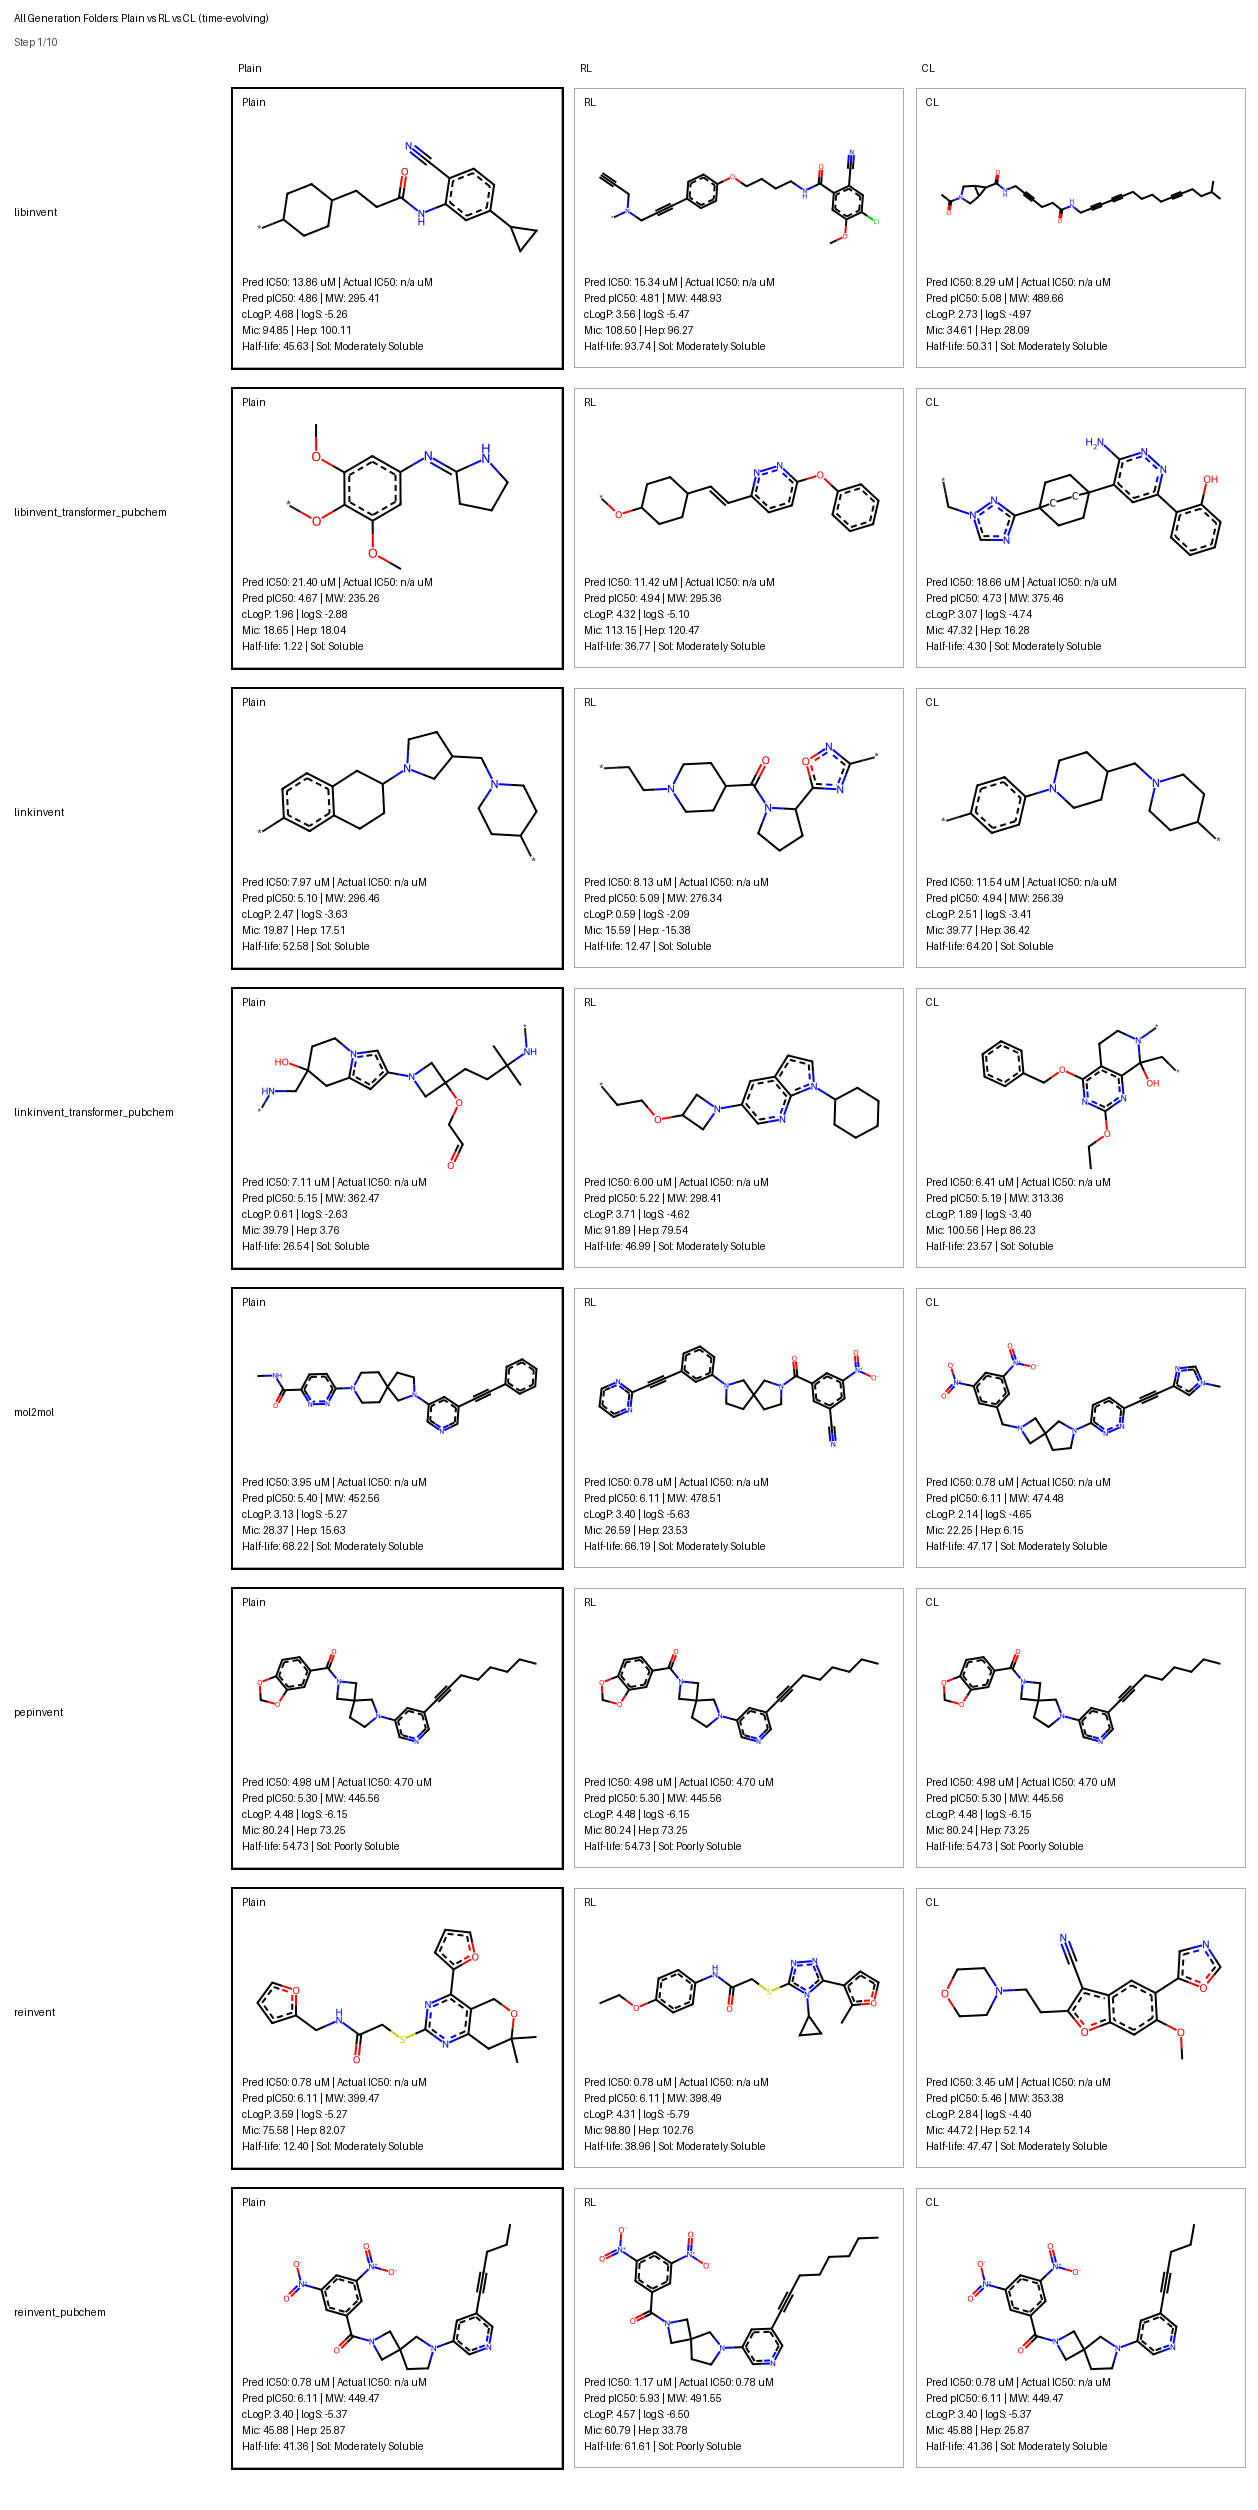
\includegraphics[width=0.92\textwidth]{../outputs/generated/animations/all_generation_folders_big_timeline_first_frame.png}
  \vspace{0.2em}

  {\small Timeline view of all generation campaign folders. \textit{(Full animation: \texttt{outputs/generated/animations/all\_generation\_folders\_big\_timeline.gif})}}
\end{frame}

% ============================================================
\begin{frame}{Top Generation Outputs: Combined View}
  \centering
  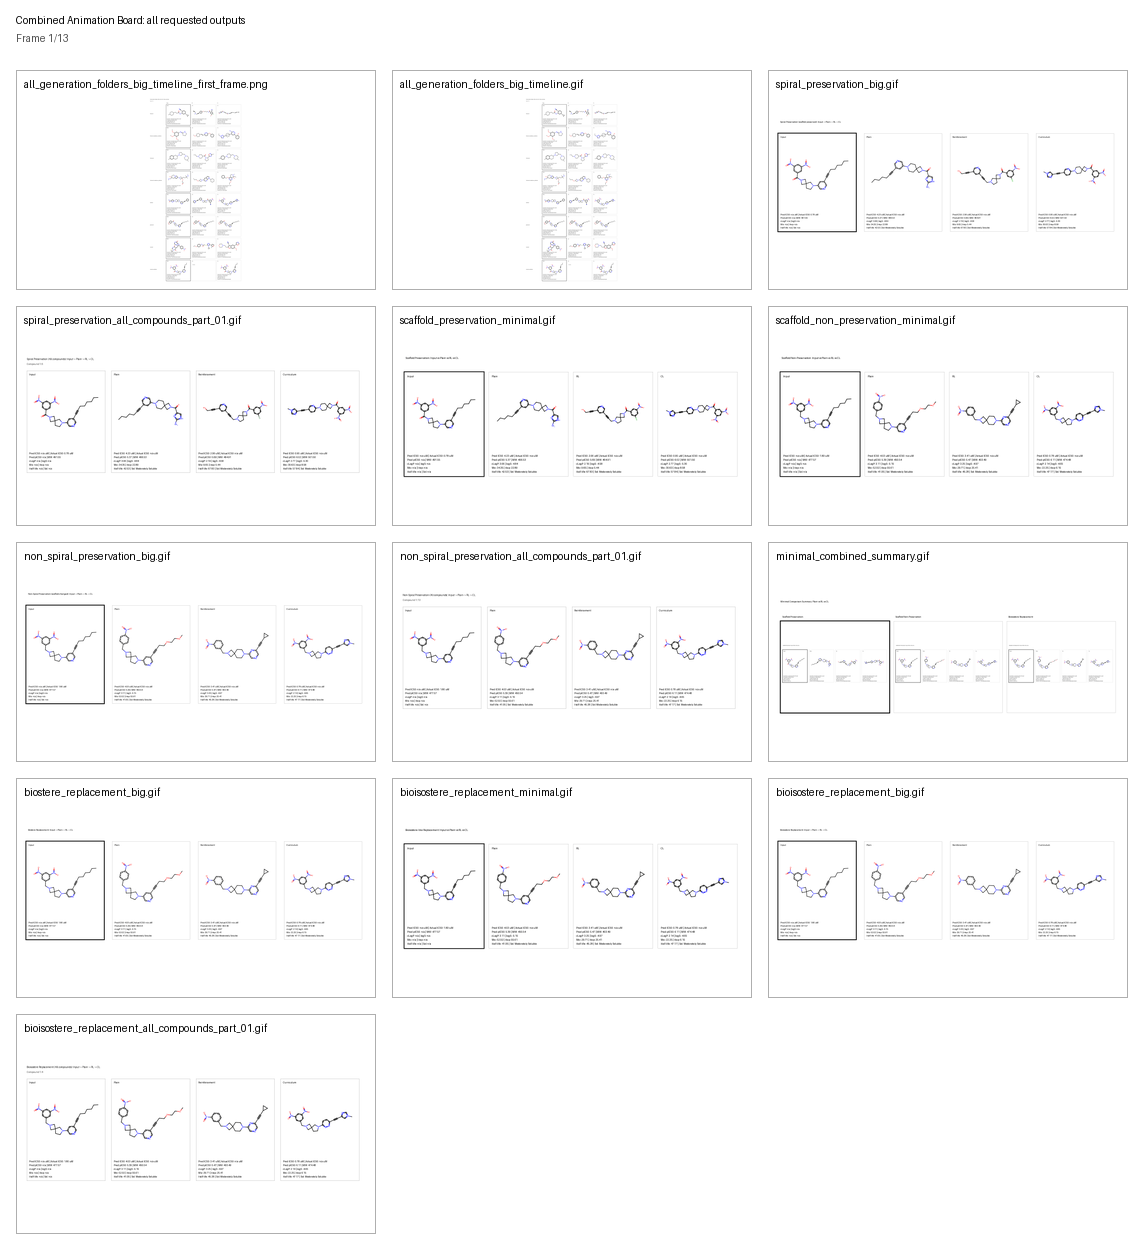
\includegraphics[width=0.90\textwidth]{../outputs/generated/animations/all_requested_outputs_combined_first_frame.png}
  \vspace{0.2em}

  {\small Combined animation of 13 output assets across all generation families and modes. \textit{(Full GIF: \texttt{all\_requested\_outputs\_combined.gif})}}
\end{frame}

% ============================================================
\begin{frame}{End-to-End Generation Pipeline: Phase Overview}
  \centering
  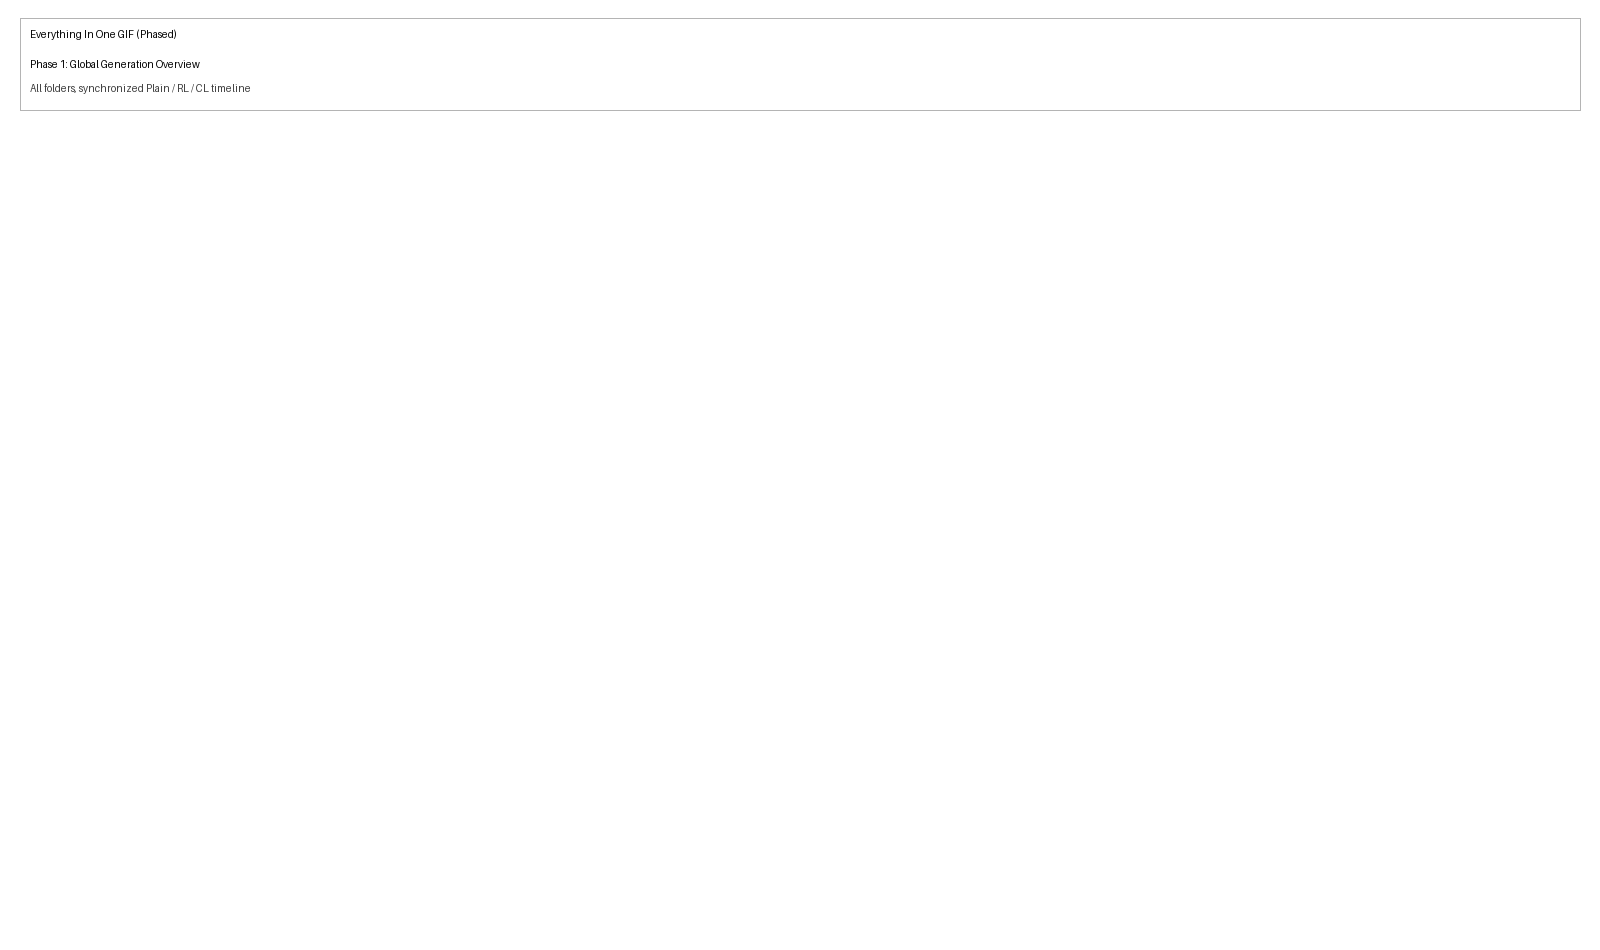
\includegraphics[width=0.90\textwidth]{../outputs/generated/animations/everything_in_one_with_phases_first_frame.png}
  \vspace{0.2em}

  {\small 9-phase end-to-end pipeline summary across all generation modes (78 total frames). \textit{(Full GIF: \texttt{everything\_in\_one\_with\_phases.gif})}}
\end{frame}

% ============================================================
\begin{frame}{Selected Folders: Detailed Output}
  \centering
  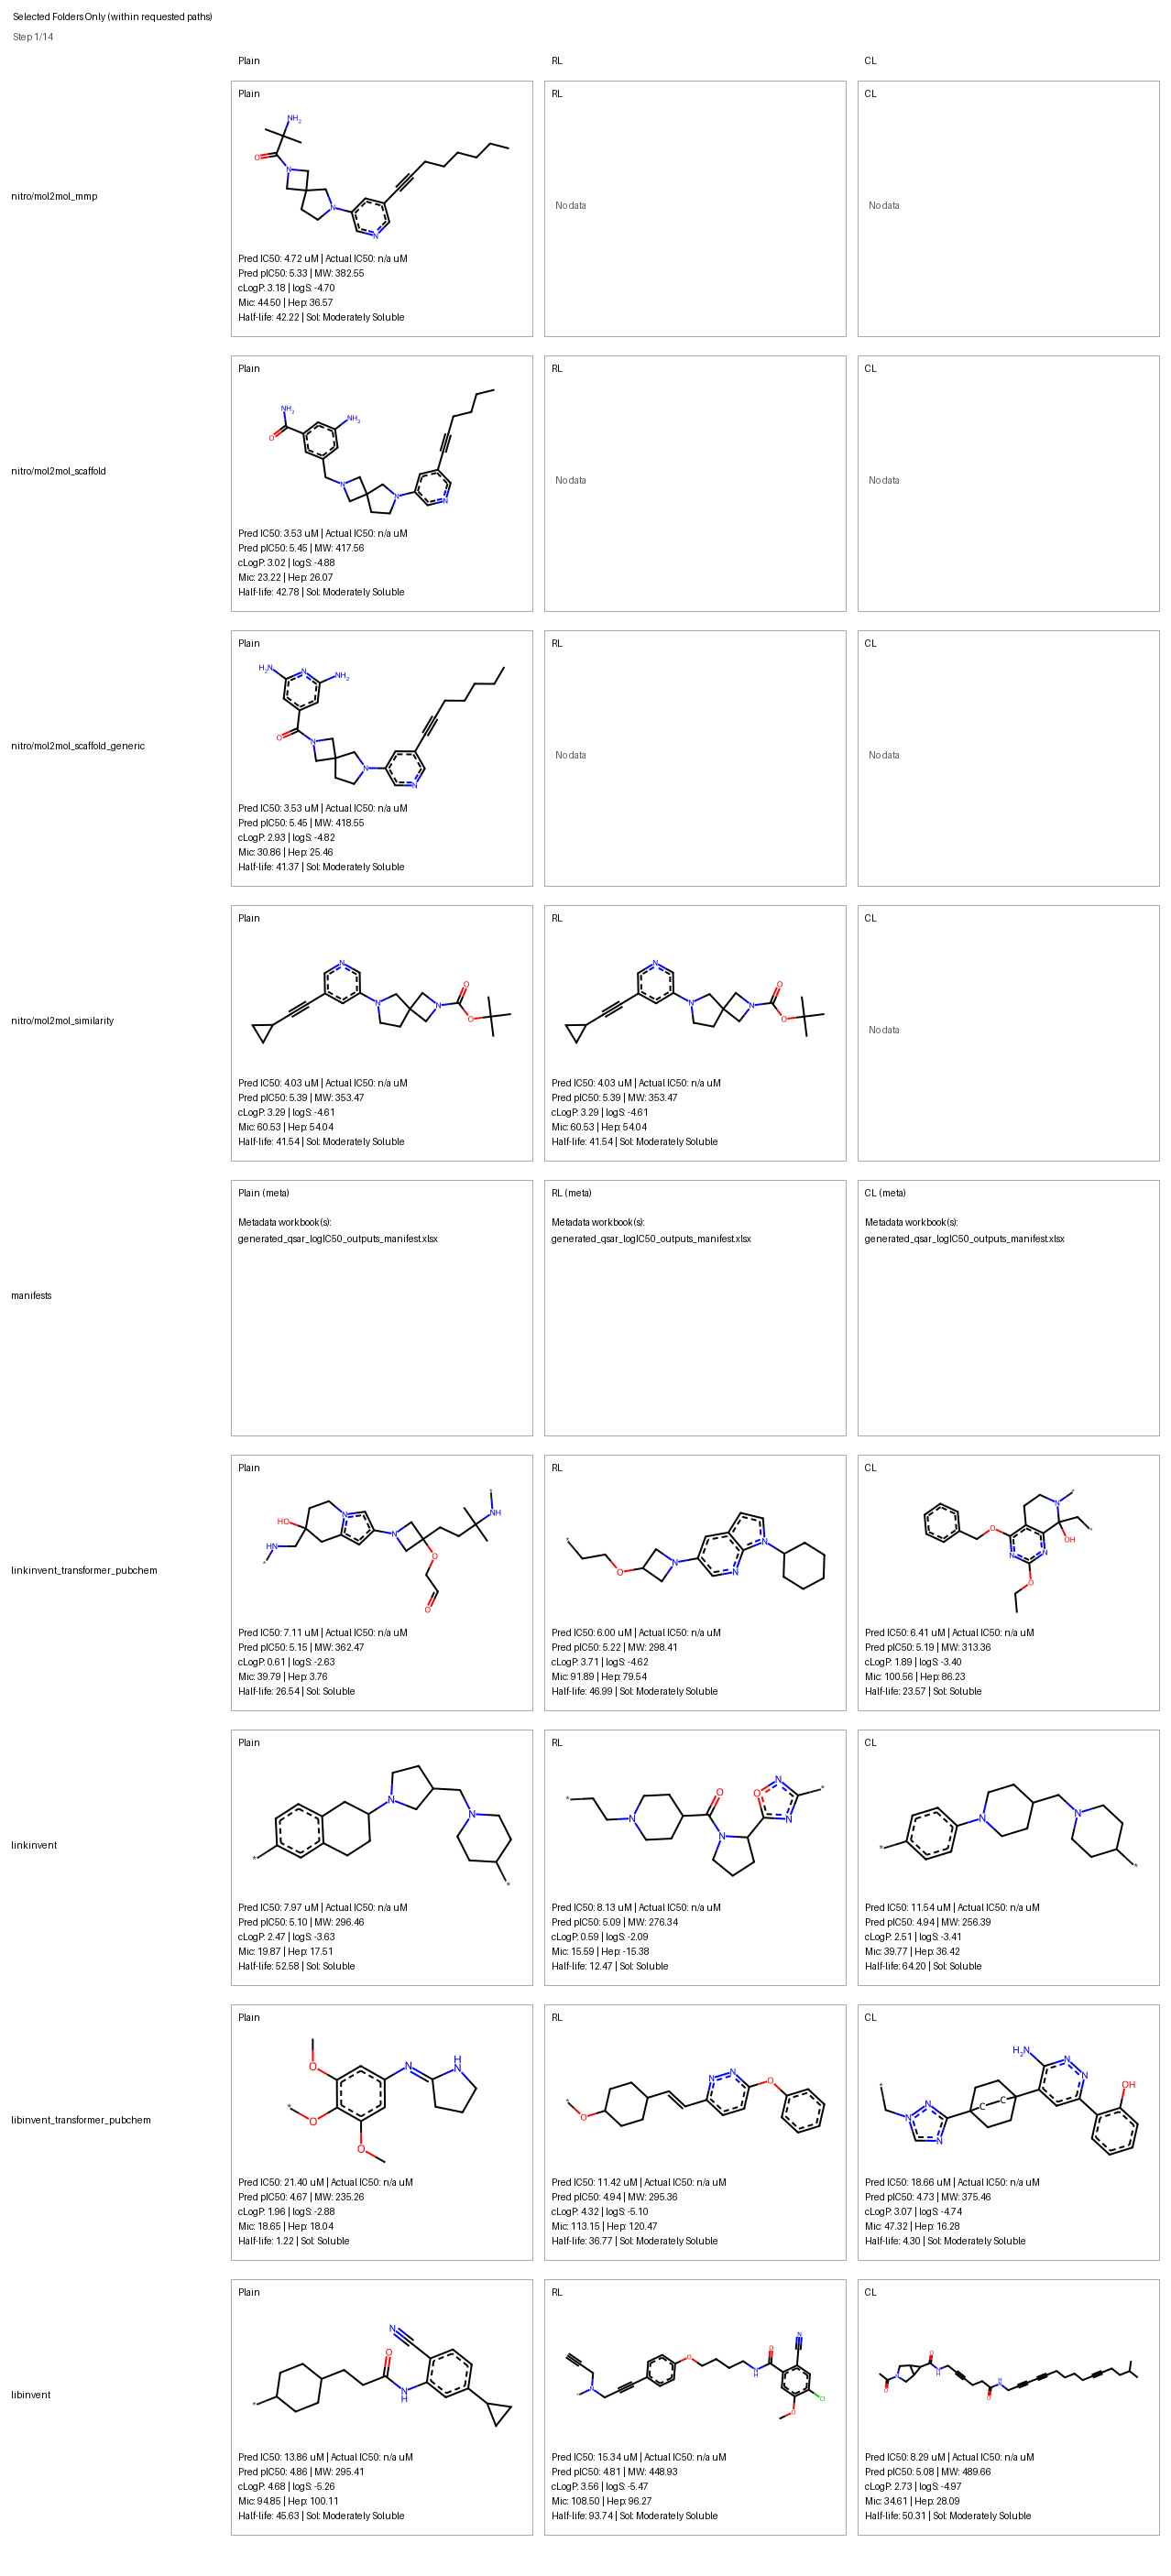
\includegraphics[width=0.90\textwidth]{../outputs/generated/animations/selected_folders_within_first_frame.png}
  \vspace{0.2em}

  {\small Detailed compound visualisation within selected generation folders. \textit{(Full GIF: \texttt{selected\_folders\_within.gif})}}
\end{frame}

% ============================================================
\section{Summary}

\begin{frame}{Summary: QSAR Model Performance}
  \centering
  \small
  \begin{tabular}{lll}
    \toprule
    \textbf{Metric} & \textbf{Value} & \textbf{Context} \\
    \midrule
    Primary model          & RDKit + KNN     & Highest CV R$^2$ \\
    CV R$^2$               & 0.887           & Excellent for low-data QSAR \\
    Test MAE (Series C)    & 0.118 pIC$_{50}$ & $\approx$32\% IC$_{50}$ error \\
    Test R$^2$ (Series C)  & 0.887           & 5 measured compounds \\
    Series E predictions   & 7.38 -- 34.11\,$\mu$M & 6 prospective compounds \\
    Ensemble models        & 4 additional    & Uncertainty estimation \\
    \bottomrule
  \end{tabular}
  \vspace{0.5em}

  \begin{columns}
    \column{0.48\textwidth}
    \begin{block}{Generation Campaign}
      \small
      \begin{tabular}{lc}
        Total candidates   & 37,451 \\
        Gate~1 shortlisted & 200 \\
        Unique scaffolds (Gate~1) & 155 \\
        ADME-passing       & 65 (33\%) \\
        Best pred IC$_{50}$ & 0.78\,$\mu$M \\
        Best triage score  & 0.921 \\
      \end{tabular}
    \end{block}
    \column{0.48\textwidth}
    \begin{alertblock}{Recommended Next Steps}
      \small
      \begin{enumerate}
        \item Synthesise top 65 ADME-passing Gate~1 compounds
        \item Measure IC$_{50}$ vs.\@ Mtb H37Rv
        \item Re-train QSAR with new data (Series C + E + Gate~1 actives)
        \item Iterate: run new generative campaign seeded with confirmed actives
      \end{enumerate}
    \end{alertblock}
  \end{columns}
\end{frame}

% ============================================================
\begin{frame}{All Prediction Measurements at a Glance}
  \centering
  \small
  \begin{tabular}{p{3.8cm}p{3.0cm}p{4.5cm}}
    \toprule
    \textbf{Measurement} & \textbf{Gate~1 Range} & \textbf{Description} \\
    \midrule
    pred\_pIC50           & 4.94 -- 6.11          & Primary potency prediction \\
    pred\_ic50\_uM        & 0.78 -- 11.55\,$\mu$M & IC$_{50}$ in micromolar \\
    pred\_cLogP           & 1.93 -- 2.80           & Lipophilicity (Crippen) \\
    pred\_logS\_ESOL      & $-$5.34 to $-$3.51    & Aqueous solubility (log mol/L) \\
    pred\_MetStab\_CL\_Microsome & --- & Microsomal clearance (AZ model) \\
    pred\_MetStab\_CL\_Hepatocyte & --- & Hepatocyte clearance (AZ model) \\
    adme\_individual\_score & 0.70 -- 0.94         & Composite ADME scoring \\
    triage\_score         & 0.77 -- 0.92           & Final composite ranking \\
    Tanimoto              & 0.28 -- 0.86           & Similarity to training set \\
    pred\_pIC50\_uncertainty & 0 (current run)     & Ensemble std ($\sigma$ predictions) \\
    \bottomrule
  \end{tabular}
  \vspace{0.5em}
  {\small\textit{All predictions generated by the primary RDKit+KNN QSAR model and AZ ADME models. IC$_{50}$ uncertainty requires a re-run with full ensemble enabled.}}
\end{frame}

% ============================================================
\begin{frame}[plain]
  \centering
  \vspace{2cm}
  {\Huge \textbf{Thank You}}\\[1em]
  {\large QSAR-Guided Generative Design for TB Drug Discovery}\\[0.5em]
  {\normalsize March 2026}\\[1.5em]
  \begin{tabular}{ll}
    Primary model:  & RDKit + KNN, R$^2$ = 0.887 \\
    Test MAE:       & 0.118 pIC$_{50}$ (Series C) \\
    Shortlisted:    & 200 compounds from 37,451 \\
    Best predicted: & 0.78\,$\mu$M IC$_{50}$ \\
  \end{tabular}
\end{frame}

\end{document}
